\chapter{Infraestrutura}\label{chp:infraestrutura}

Para a realização da solução proposta neste trabalho, recursos de infraestrutura são necessários para que seja possível a execução de rotinas de rastreamento de contatos no servidor, utilização do BD e da comunicação entre o cliente e o servidor. Assim, na Seção \ref{sec:firebase} será explicado o que é e para que serve um serviço de \textit{backend}, quais recursos de infraestrutura serão utilizados e o que são os sistemas de autenticação e o envio de mensagens. Na Seção \ref{sec:firestore} será explicado sobre a solução de BD da plataforma \textit{Firebase} e o que cada entidade dele significa. Por fim, na Seção \ref{sec:cloudfunctions} será explicado o que é a \textit{Cloud Function} e qual será a responsabilidade dela neste projeto.

\section{Serviço de \textit{Backend}}\label{sec:firebase}

A infraestrutura da aplicação será totalmente em nuvem e os principais motivos dessa decisão foram: as faturas de cobrança estão diretamente relacionadas à carga de utilização, e como o escopo deste trabalho é um teste de conclusão de curso, essa carga será baixa; totalmente gerenciado por grandes empresas; boa documentação e facilidade na criação de ambientes.

A nuvem que será utilizada neste trabalho é a \Sigla{\textit{Google Cloud Platform}}{GCP} porque ela entrega serviços que atendem perfeitamente os requisitos do trabalho, por exemplo, APIs de busca de locais que utilizam o BD do \textit{Google}.

Neste projeto será utilizado um \Sigla{\textit{Backend-as-a-Service}}{BaaS}, que é um serviço de \textit{backend} gerenciado por uma empresa. Como a provedora de nuvem escolhida nesse projeto é a GCP, o serviço de BaaS dela se chama \textit{Firebase}.

\textit{Firebase} é uma plataforma digital que tem como objetivo acelerar o processo de desenvolvimento de aplicativos e oferecer serviços que atendam diversos requisitos, como a criação de BDs escaláveis, sistemas de autenticação, sistemas de envio de notificações, entre outros serviços.

O \textit{Firebase} está diretamente relacionado com a GCP. Todo projeto criado nele também está representado na GCP, que é a base dos serviços de computação em nuvem da \textit{Google}. A diferença é que o \textit{Firebase} abstrai grande parte da configuração da infraestrutura, gerenciando as configurações necessárias para que os serviços funcionem automaticamente, sem que o usuário precise entender sobre cada detalhe que acontece em segundo plano.

Alguns serviços existem nas duas plataformas, e no fundo são os mesmos, apenas com interfaces de consumo diferentes. Por exemplo, o serviço de \textit{Cloud Functions} pode ser utilizado em ambas plataformas, e quando criado no \textit{Firebase}, também é possível visualizá-lo na interface da GCP.

Porém, algumas configurações não são possíveis de serem feitas diretamente pelo \textit{Firebase}. Um exemplo disso é a gestão de identidades, que é responsável por definir quais permissões cada usuário tem dentro da plataforma e só pode ser configurada pela GCP.

A principal vantagem competitiva do \textit{Firebase} quando comparado a outras plataformas é a alta produtividade que ele traz ao desenvolvimento de aplicativos.

Os serviços do \textit{Firebase} que serão utilizados neste trabalho são o sistema de autenticação, o envio de notificações, o BD e as \textit{Cloud Functions}.

Começando pela autenticação, ela é a peça chave para que os locais visitados pelos usuários sejam salvos em seus respectivos documentos no BD, dando uma experiência personalizada no aplicativo. Essa autenticação pode ser feita de diversas formas diferentes, algumas delas são o \textit{login} utilizando \textit{e-mail} e senha, número de telefone celular, redes sociais e autenticação anônima.

A autenticação anônima, que é o único método de autenticação utilizado pelo aplicativo, é criado pelo próprio \textit{Firebase}. Ela é necessária somente para que o aplicativo diferencie os usuários para efetuar o rastreamento, sem precisar de informações pessoais do mesmo.

Outro serviço que será utilizado é o \Sigla{\textit{Firebase Cloud Messaging}}{FCM}, que é responsável pelo envio de notificações aos usuários que forem possivelmente expostos à alguma doença infecciosa.

O FCM é bastante flexível e possui algumas funcionalidades que atendem diferentes casos de uso. A principal funcionalidade são as formas que a notificação pode ser enviada para o cliente, que são para dispositivos únicos, grupos de dispositivos ou para os dispositivos inscritos em tópicos. 

O envio de notificações deve ser feito de forma automática, para isso, os outros 3 recursos de infraestrutura trabalharão em conjunto para que a implementação da lógica do envio de mensagens seja feita com sucesso.

\section{\textit{Firestore}}\label{sec:firestore}

O \textcite{FirestoreDocs} é um BD não relacional orientada a documentos oferecido pela \textit{Google}. As principais características dele são:

\begin{itemize}
    \item \textit{Serverless}: sem servidor, totalmente gerenciado por tecnologias da Google e com escalonamento automático para atender qualquer carga de requisições;
    \item Mecanismo de consulta avançado: permite a execução de transações com \Sigla{Atomicidade, Consistência, Isolamento e Durabilidade}{ACID} nos dados dos documentos armazenados;
    \item Segurança: integração com a autenticação do \textit{Firebase} para possibilitar controles de acesso de segurança com base na identidade;
    \item Replicação multirregional: redundância de BD em diversos \textit{data centers} espalhados pelo mundo com alta consistência, aumentando a disponibilidade do serviço, mesmo em caso de desastres;
    \item Flexibilidade: o modelo de dados disponibiliza a criação de estruturas hierárquicas flexíveis, onde os dados são armazenados em documentos, e estes organizados em coleções;
    \item Integração: o \textit{Firestore} possui integração perfeita com outros produtos do \textit{Firebase} ou da GCP.
\end{itemize}

O modelo de dados do \textcite{FirestoreDataModel} segue o formato JSON e é estruturado em entidades denominadas documentos e coleções. A \Figura{fig:exemplofirestorejson} demonstra um exemplo dessa estrutura.

\begin{figure}[!htb]
    \centering
    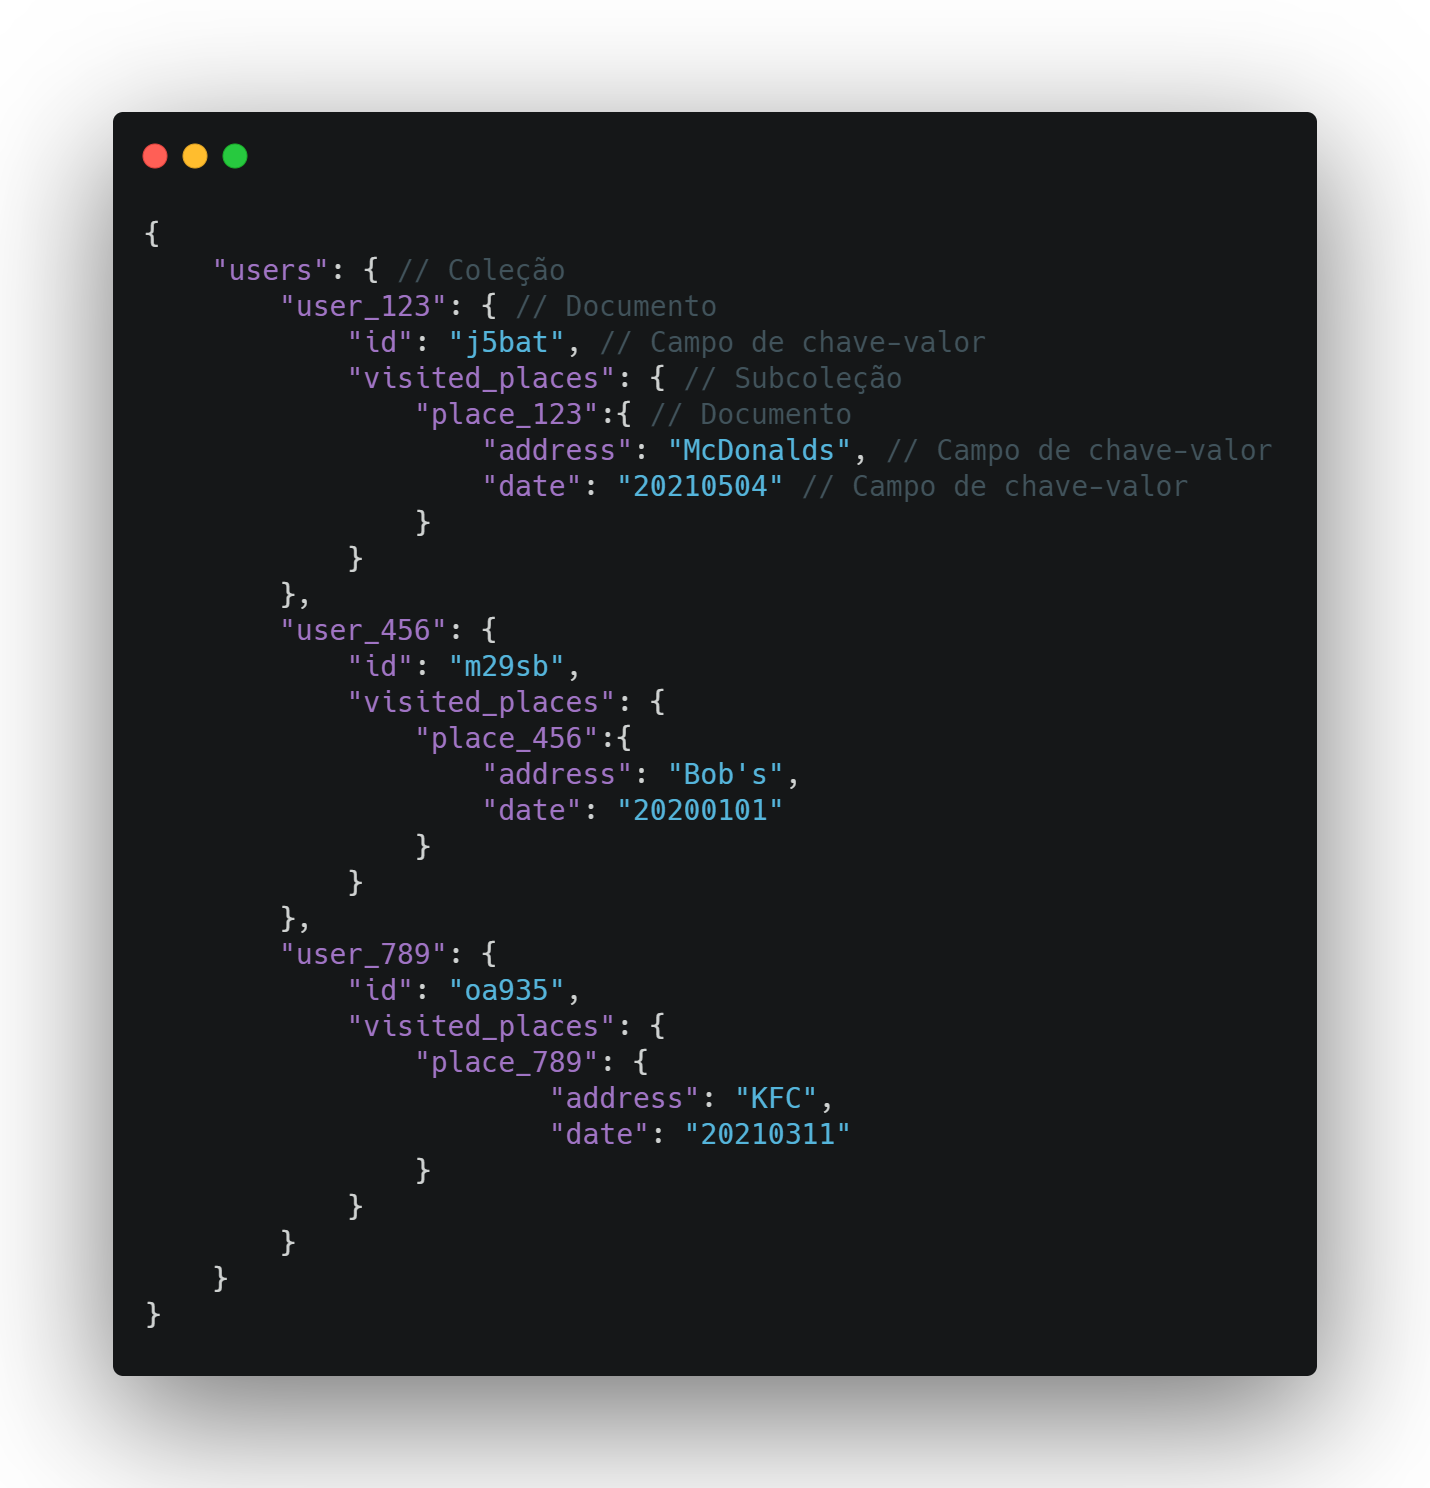
\includegraphics[scale=0.3]{Estrutura Firebase JSON - Carbon Code (estilo Seti).png}
    \caption{Exemplo de estrutura JSON com anotações referentes ao \textit{Firestore}.}
    \label{fig:exemplofirestorejson}
\end{figure}

Documento é a unidade de armazenamento do \textit{Firestore}, com campos que são mapeados para valores. Esses valores podem ser de diversos tipos: números inteiros, booleanos, \textit{timestamps}, \textit{strings} e até estruturas de dados como listas e mapas.

Cada documento é identificado por um nome e não podem possuir outros documentos criados diretamente dentro dele.

Como o \textit{Firestore} não possui nenhum esquema, o desenvolvedor tem total liberdade sobre quais campos colocar em cada documento e quais tipos de dados esses campos armazenam.

Utilizando os mesmos valores e estrutura da \Figura{fig:exemplofirestorejson}, a \Figura{fig:explicacaodocumentofirestore} representa um exemplo de documento do \textit{Firestore}.

\begin{figure}[!htb]
    \centering
    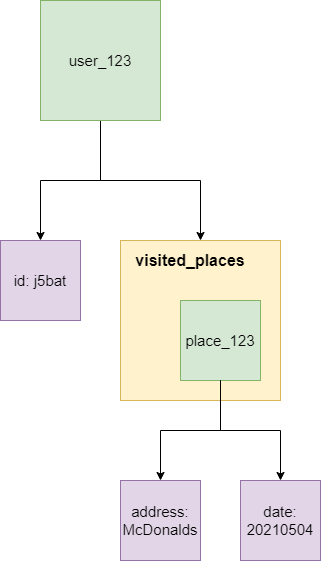
\includegraphics[scale=0.6]{documento-firestore.png}
    \caption{Exemplo de documento do \textit{Firestore}.}
    \label{fig:explicacaodocumentofirestore}
\end{figure}

As coleções são recipientes que armazenam um conjunto de documentos e são referenciadas pelo seu nome, da mesma forma que os documentos.

Os documentos dentro das coleções devem ter identificadores únicos, ou seja, dois documentos diferentes não podem possuir o mesmo nome dentro da mesma coleção. Por conta disso, é comum que os documentos sejam nomeados com o \Sigla{Identificador}{ID} do objeto que ele representa.

É importante ressaltar que coleções não podem armazenar dados diretamente, apenas através de documentos. Seguindo o mesmo raciocínio, os documentos não podem armazenar outros documentos. Cada entidade possui responsabilidades específicas. Por conta disso, para criar uma estrutura hierárquica no \textit{Firestore}, as coleções armazenam exclusivamente documentos, e os documentos, além dos campos chaves-valor, podem armazenar subcoleções - que possuem as mesmas características de uma coleção.

Para melhor visualização da estrutura hierárquica do \textit{Firestore}, a estrutura da \Figura{fig:exemplofirestorejson} está representada na \Figura{fig:explicacaofirestorecompleto}.

\begin{figure}[!htb]
    \centering
    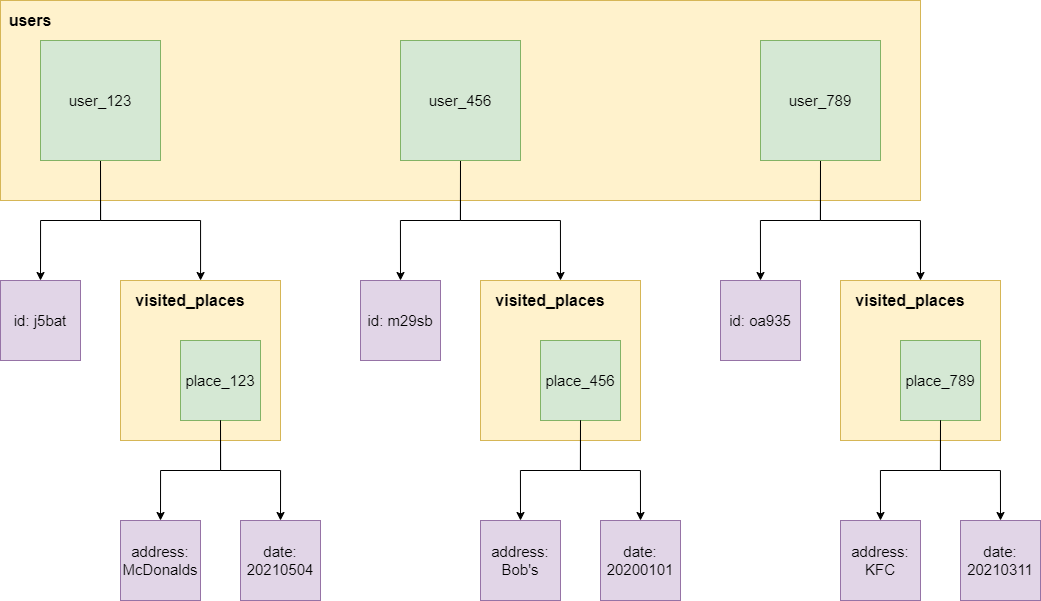
\includegraphics[scale=0.43]{Estrutura Firestore.png}
    \caption{Exemplo de estrutura hierárquica do \textit{Firestore}}
    \label{fig:explicacaofirestorecompleto}
\end{figure}

\section{\textit{Cloud Functions}}\label{sec:cloudfunctions}

A \textit{Cloud Function} é o produto de função como serviço para criar aplicações com base em eventos, disponibilizado pelas plataformas \textit{Firebase} e GCP. Ela é uma maneira de ampliar o comportamento de um aplicativo e integrar com outros recursos disponíveis na plataforma por meio da adição de código no servidor. Com base nisso, ela serve como camada conectiva, disponibilizando a construção de lógicas entre os serviços da plataforma por meio da detecção e da resposta a eventos.

No caso de uso deste trabalho, a \textit{Cloud Function} consome os eventos de escrita em coleções específicas no \textit{Firestore}, tratando-os através da execução do trecho de código implementado na função.
